\section*{Источники и решения}

Это классическая теорема, простая и удивительная; о ней мне напомнил Дэн Ромик, сейчас он в Иерусалимском университете.
В третьем томе своего «Искусства программирования» \cite{knut} Дональд Кнут проследил историю этого результата до сноски в книге 1955 года Германа Бёрнера \cite{boerner}.
Бриджет Теннер, студентка знаменитого комбинаторика Ричарда Стэнли из Массачусетского технологического института, недавно обобщила эту теорему \cite{tenner}.
Теорему Бёрнера --- одна из задач, где таинственность и очевидность чередуются при каждой попытке найти решение.

Предположим, что матрица имеет $m$ строк и $n$ столбцов.
Положим, что $a_{ij}$ --- значение $i$-й строке и $j$-м столбце матрицы
после упорядочивания каждой строки (будем считать, что самые маленькие значения находятся слева).
Обозначим через $b_{ij}$ значение в той же клетке матрицы после упорядочивания столбцов.

Нужно показать, что $b_{ij} \le b_{ik}$ если $j < k$.
Заметим, что $b_{ik}$ это $i$-й наименьший элемент в старом столбце $\{a_{1k}, a_{2k}, \dots, a_{mk}\}$.
Далее, $a_{i'j}\le a_{i'k}$ поскольку $a_{i'j}$ стоит левее $a_{i'k}$ в той же строке.
В частности, если $a_{i'k}\le b_{ik}$, то $a_{i'j}\le b_{ik}$.
Значит есть как минимум $i$ элементов из старого $j$-го столбца, которые не превосходят $b_{ik}$,
и в частности, $i$-й наименьший элемент в старом $j$-м столбце не превосходит $b_{ik}$;
то есть, $b_{ij} \le b_{ik}$ --- конец доказательства.

Может убедительней разобрать конкретный пример?
Решайте сами.


\begin{addedbytheeditors}
\textbf{Редакторам:} Перетащил одну фразу из одного абзаца в другой.
\end{addedbytheeditors}

\subsection*{Нежелательное раскрытие}

Эта любопытная головоломка была передана мне Ричардом Липтоном из Колледжа вычислительной техники в Джорджии.
Выражение можно проанализировать с точки зрения глубины деревьев, но есть и более простой способ:
установите все переменные равными 2!
Поскольку применение закона дистрибутивности не меняет значения выражения,
получаем ограничение на длину любого выражения которое можно получить из него раскрывая скобки.

\subsection*{Хамелеоны}

Борис Шейн, алгебраист из Университета Арканзаса, прислал мне эту головоломку; она может быть довольно древней.
Мне известен случай когда её дали ученику восьмого класса в Харькове,
и ещё другой, когда её дали выпускнику Гарварда, проходившему собеседование в крупной финансовой фирме;
оба с ней справились!

Главное увидеть, что после каждой встречи пары хамелеонов разница между числом особей любых двух цветов не меняется по модулю~3.
Обозначим через $N_{\text{к}}$ число красных хамелеонов, аналогично
$N_{\text{с}}$ и $N_{\text{з}}$ --- число синих и зелёных;
мы утверждаем, что, например, у $N_{\text{к}} - N_{\text{с}}$ не меняется остаток при делении на~$3$ после каждой встречи хамелеонов.
В этом можно убедиться проверив случай за случаем.
Таким образом, эти разницы остаются одинаковыми по модулю 3 навсегда, и поскольку на острове ни одна из этих разниц не равна нулю по модулю 3, нам никогда не удастся избавится от обоих этих цветов.

С другой стороны, одна из этих разниц (скажем, $N_{\text{к}} - N_{\text{с}}$) является положительным кратным $3$, то её можно уменьшить, заставив красного хамелеона встретиться с зелёным (если зелёных нет, то придётся сначала заставить красного встретиться с синим).
Повторив это несколько раз, можно добиться, что $N_{\text{к}} = N_{\text{с}}$.
Затем заставим красных хамелеонов встречаются синими, пока не останутся только зелёные.
Собрав всё воедино и отметив, что если две разницы кратны $3$, то и третья кратна $3$, мы увидим, следующее:
\begin{itemize}
\item если все три разницы кратны 3, то любой цвет может захватить остров;
\item если только одна из разниц кратна 3, то оставшийся цвет --- единственный, который может захватить остров; и наконец,
\item если ни одна из разниц не кратна 3, как в данной задаче, то все хамелоны не смогут стать одноцветными, до тех пор, пока не вмешаются другие обстоятельства (например, рождение или смерть).
\end{itemize}

Эта головоломка была предложена осенью 1984 года на Турнире городов (с числами 13, 15 и 17);
задача 5 в подготовительном варианте для 9--10 классов и основном варианте для 7--8 классов.
Турнир городов, из которого будут ещё задачи, был основан в 1980 году Николаем Константиновым из Москвы.
В то время начиналась перестройка и гласность, это затронуло и математические олимпиады, как и все другие аспекты советской жизни.
Константинов был недоволен определёнными переменами, ушёл из Центрального жюри и сам организовал турнир для маленьких городов в сельской России.
Он собрал вокруг себя ядро выдающихся математиков, и успех турнира в конечном итоге привёл к тому, что Москва сама стала одним из «городов».
Эта же группа основала Независимый московский университет в 1993 году.
Сама же группа превратилась в МЦНМО.

Турнир распространился в Польшу и Болгарию, а в 1989 году --- в Австралию, благодаря усилиям Питера Тейлора из Университета Канберры.
В настоящее время Тейлор является исполнительным директором Австралийского математического фонда, под чьим патронатом он выпустил пять книг о турнире.

В 1990 году Энди Лиу привёз Турнир в Канаду.
С тех пор он распространился по всему миру, с участниками из Соединённых Штатов, Западной Европы, Азии и Южной Америки.
Английский вариант и решения подготавливаются Андреем Сторожевым и Энди Лиу.

\begin{addedbytheeditors}
\textbf{Редакторам:} Вроде история тургора не соответствует действительности.
\end{addedbytheeditors}

\subsection*{Отсутствующая цифра}

Эта забавная загадка взята из колонки головоломок Берлекэмпа и Бюлера в журнале Emissary [3], весна/осень 2006 года,
а они услышали её от теоретика чисел Хендрика Ленстры.
Конечно же можно загуглить ``\texttt{2\^{}29}'' и увидеть число, но как решить эту задачу в уме, без головной боли?

Ну возможно, вы помните технику из начальной школы, называемую вычеркиванием девяток, если сложить все цифры то получим значение числа по модулю 9 (то есть  с тем же остатком при деления на 9).
Иногда этот метод называется индуской или арабской проверкой;
он основан том, что $10 \equiv 1 \pmod 9$, следовательно, $10^n \equiv 1^n \equiv 1 \pmod 9$ для любого $n$.
Если обозначить через $x^*$ сумму цифр числа $x$, то получим $(xy)^* \equiv x^* y^* \pmod 9$ для любых $x$ и $y$.
В частности, $(2^n)^* \equiv 2^n \pmod 9$.
Остатки от деления степеней числа $2$ на $9$ начинаются с $2$, $4$, $8$, $7$, $5$, $1$, и зацикливается;
так как $29 \equiv 5 \pmod 6$, получаем, что $2^n \pmod 9$ есть пятое число этой последовательности, то есть $5$.
Теперь сумма всех цифр равна $10 \times 4{,}5 = 45 \equiv 0 \pmod 9$, поэтому пропущенная цифра должна быть четвёрткой.
И действительно, $2^{29} = 536\,870\,912$.

\subsection*{Очень честное разбиение}

Мне эту головоломку предложил Муту Мутукиршнан (Рутгерс),
а сам он услышал её от Боба Тарджана (Принстон);
оба они выдающиеся специалисты по информатике.

Оказывается, такое разбиение действительно существует: $\{1$, $4$, $6$, $7$, $10$, $11$, $13$, $16\}$ и $\{2$, $3$, $5$, $8$, $9$, $12$, $14$, $15\}$.

Чтобы догадаться как его стоить, можно подумать:
А ведь $16$ это степень двойки;
может попытаться обобщить?
Можно ли, например, разбить числа от $1$ до $8$ на две равные части с одинаковой суммой и суммой квадратов?
А как насчёт разделения чисел от $1$ до $4$ на две равные части с одинаковой суммой?
Последнее сделать легко: $\{1, 4\}$ и $\{2, 3\}$.
Заметим, что $\{5, 8\}$ и $\{6, 7\}$ разбивают числа от $5$ до $8$, решая ту же задачу.
Если соединить эти два разбиения крест-накрест, то получим $\{1, 4, 6, 7\}$ и $\{2, 3, 5, 8\}$, по построению оно подходит для сумм, но вроде бы подходит и для сумм квадратов.

В общем случае, пользуясь индукцией, можно доказать, что числа от $1$ до $2^k$ можно разбить на множества $X$ и $Y$ так, что каждая часть имеет одинаковую сумму $j$-х степеней, где $j$ меняется от $0$ до $k - 1$, и, значит $p(X)=p(Y)$ для любого многчлена $p$ степени меньше $k$;
где $p(X)$ определятся как сумма всех $p(x)$ при $x \in X$.

Чтобы перейти от $2^{k}$ к $2^{k+1}$, возьмём $X' = X \cup (Y + 2^k)$
(где $Y + 2^k$ получается из $Y$ добавлением $2^k$ к каждому элементу) и $Y' \z= Y \cup (X + 2^k)$.
Заметим, что $p(X + 2^k) = p(Y + 2^k)$,
так как $p(X + 2^k)=q(X)$ и $p(Y + 2^k)=q(Y)$ для некоторого другого многчлена $q$ той же степени.
Таким образом, $X'$ и $Y'$ согласуются для многчленов степени меньше $k$, ну а что если наш многочлен $r$ степени $k$?

Но и здесь всё в порядке, ведь старшие члены в $r(x+2^k)$ и $r(x)$ совпадают;
то есть $s(x)=r(x+2^k)-r(x)$ есть многочлен степени меньше $k$.
Таким образом,
\begin{align*}
r(X')&=r(X)+r(Y+2^k)=r(X)+r(Y)+s(Y),
\\
r(Y')&=r(Y)+r(X+2^k)=r(Y)+r(X)+s(X).
\end{align*}
Поскольку $s(Y)=s(X)$, получаем, что $r(X')\z=r(Y')$.


\begin{addedbytheeditors}
\textbf{Редакторам:} Я расширил последний параграф.
\end{addedbytheeditors}

\subsection*{Восстановление чисел}

Эту головоломку прислал мне Ник Райнгольд из AT\&T Labs.
Ответ таков: это возможно тогда и только тогда, когда $n$ не является степенью двойки!
И мы снова применим силу многочленов.

Предположим, что $X = \{x_1 , \dots , x_n\}$ и $Y = \{y_1 , \dots , y_n\}$ --- два различных множества с одинаковыми попарными суммами.
Пусть $p(z)$ --- многочлен $z^{x_1} + z^{x_2} + \dots + z^{x_n}$,
а $q(z)$ --- многочлен $z^{y_1} + z^{y_2} + \dots + z^{y_n}$.
По условию, смешанные члены в $p(z)^2$ те же, что и в $q(z)^2$;
то есть,
\[p(z)^2 -q(z)^2 = p(z^2 )-q(z^2).\]
Разделив равенство на $p(z) - q(z)$, получим
\[p(z) + q(z) =
\frac{p(z^2 ) - q(z^2 )}{p(z) - q(z)}.
\]
Поскольку $p(1) = q(1) = n$,
У многочлена $p(z) - q(z)$ есть корень 1 с некоторой положительной кратностью $k$.
Значит
\[p(z) - q(z) = (z - 1)^k r(z).\]
Аналогично 
\[p(z^2 ) - q(z^2 ) = (z^2 - 1)^k r(z^2 )= (z - 1)^k (z + 1)^k r(z^2).\]
Сократив дробь на $(z - 1)^k$ получаем
\[p(z) + q(z) =
\frac{(z + 1)^k r(z^2)}{r(z)}.
\]
Подставив $z = 1$, получаем $2n = 2^k$ --- пол дела сделано!

Остаётся показать, что не всегда возможно восстановить целые числа, когда $n$ является степенью двойки.
Для этого воспользуемся множествами $X$ и $Y$ из предыдущей задачи.
Предположим, что $X$ и $Y$ разбивают $\{1, \dots , 2^k\}$ давая те же парные суммы.
Рассмотрим $X' = X \cup (Y + 2^k)$ и $Y' = Y \cup (X + 2^k)$.
Парные суммы $X'$ имеют вид $x_1 + x_2$ , $y_1 + y_2 + 2^{k+1}$ , и $x + y + 2^k$.
По предположению индукции,
суммы $x_1 + x_2$, те же, что $y_1 + y_2$.
Значит, попарные суммы из $Y'$ точно те же, что из $X'$.

\begin{addedbytheeditors}
Про пример можно думать геометрически.
Если $X$ и $Y$ --- множества чётных и нечётных вершин $k$-мерного параллелепипеда, то легко видеть, что все середины диагоналей с вершинами в $X$ те же, что с вершинами в $Y$.
Остаётся спроектировать параллелепипед на прямую так чтоб все вершины попали в целые числа.
\end{addedbytheeditors}

\subsection*{Уравнение ирисок}

Эта задача была представлена Клиффом Смитом (MIT) на прекрасном сайте головоломок \cite{bohman-pikhurko-frieze-sleator}, который ведут Том Боман, Олег Пихурко, Алан Фриз и Дэнни Слейтор в Университете Карнеги — Меллона.
Она появилась на Пекинском математическом соревновании старших классов 1962 года (12 класс, лист II, задача 4).

Пусть $M$ --- максимальное число ирисок у одного из детей в данный момент времени.
Заметим что число $M$ может увеличиться только если оно нечётное;
в этом случае оно может увеличиться только на единицу до следующего чётного числа.
Чтобы понять это, предположим сначала, что $M$ чётное; тогда оно, конечно же, не изменится, когда учитель раздаёт дополнительные ириски, а после передачи ирисок ни один ребёнок не сможет иметь их больше чем $\tfrac12 M + \tfrac12 M = M$ штук.
Если же $M$ нечётное, то оно увеличится на один до следующего чётного числа, и после этого заработает предыдущее рассуждение.

Значит, рано или поздно, учитель прекратит раздавать ириски.
Теперь наша задача --- показать, что ириски \emph{уравнятся}.

Хороший способ измерить \emph{неравенство} набора из $n$ чисел с фиксированной суммой --- рассмотреть сумму их квадратов; она минимизируется, когда числа как можно ближе стоят друг к другу.
Давайте рассмотрим этот параметр в нашем случае, а именно 
\[S = G^2_1 + G^2_2 + \dots + G^2_n,\]
где $G_i$ --- число ирисок, у $i$-го ребёнка.
Изменение $S$ после передачи ирисок составит
\begin{align*}
\left(\tfrac{1}{2}(G_n+G_1)\right)^2+\left(\tfrac{1}{2}(G_1+G_2)\right)^2+&\dots+\left(\tfrac{1}{2}(G_{n-1}+G_n)\right)^2-
\\
-G_1^2-G_2^2-&\dots-G_n^2=
\\
=-\tfrac12\bigl((G_n-G_1)^2+(G_1-G_2)^2+&\dots+(G_{n-1}-G_n)^2\bigr);
\end{align*}
это отрицательное целое число (ведь все $G_i$ сейчас уже чётные) если есть пара соседей с разным числом ирисок.
Таким образом, $S$ уменьшается каждый раз при передаче ирисок, пока число ирисок не уравнится.
Поскольку положительное число $S$ не может бесконечно уменьшаться на целые числа, всё доказано!

\subsection*{Девяносто девятая цифра}

Эта загадка взята из Emissary \cite{berlekamp-buhle}, осень 1999 года, и выглядит довольно сложной.
Даже если пользоваться компьютером, понадобится некоторое терпение (или специальная программа).

Вместо этого заметьте, что число
\[(1+\sqrt{2})^{500}+(1-\sqrt{2})^{500}\]
целое.
Ведь после раскрытия скобок, все нечётные степени $\sqrt{2}$ сокращаются.
Второе слагаемое чрезвычайно мало --- поскольку $|1-\sqrt{2}|\z<\tfrac12$, получаем $(\tfrac12)^5<0{,}1$, и, значит, оно гораздо меньше, чем $10^{-100}$ (на самом деле что-то около $4 \times 10^{-192}$).

То есть у $(1+\sqrt{2})^{500}$ нахватает крошечной величины до целого, и значит его десятичная запись обладает внушительной последовательностью девяток после запятой.
(На самом деле их $191$, и за ними следует $590591051\dots$)
В частности, 99-ой цифрой будет девятка.

Фокус добавления $(1-\sqrt{2})^{500}$ может показаться немного из ниоткуда, но такие пары сопряжённых степеней, одна большая и одна маленькая, часто встречаются в математике.
Известная формула Бине
\[F_n=\frac{1}{\sqrt{5}}\left(\frac{1+\sqrt{5}}2\right)^n-\frac{1}{\sqrt{5}}\left(\frac{1-\sqrt{5}}2\right)^n\]
выдаёт точные значения числел Фибоначчи $1, 1, 2, 3, 5, 8, 13, 21, 34 \dots$
Второе слагаемое в формуле настолько мало, что для любого $n \ge 0$ достаточно вычислить
\[\frac{1}{\sqrt{5}}\left(\frac{1+\sqrt{5}}2\right)^n;\]
тогда, округлив до ближайшего целого, получим в точности $F_n$.

\begin{addedbytheeditors}
\textbf{Редакторам:}
Я убрал следующий абзац --- по-моему он бессмысленный.

Странно, не так ли?
По тому же рассуждению $(1+\sqrt{2})^{502}$ также невероятно близко к целому,
а отношение этих двух огромных степеней равно $(1+\sqrt{2})^{2}$, что равно прозаическому  $5{,}82842712\dots$
\end{addedbytheeditors}

\subsection*{Подмножества с ограничениями}

Все три головоломки решаются одним способом.
Первая была представлена давним мастером головоломок Соломоном Голомбом (Университет Южной Калифорнии) на конференции
«Ga\-the\-ring for Gard\-ner VII»;
вторая предложена Прасадом Тетали из Технологического института Джорджии;
третья --- нехитрая её вариация.

Идея в том, чтоб покрыть числа от 1 до 30 группами чисел так, чтобы из каждой группы только одно число можно было бы включить в множество.
Если при этом получится собрать подмножество с одним элементом из каждой группы, то оно будет максимальным.

В первом случае рассмотрим любое число $k$ без квадратов (то есть его разложение содержит не больше одной копии любого простого числа).
Теперь посмотрим на множество $S_k$, которое получается, умножением $k$ на все возможные квадраты.

Если взять два числа, скажем, $kx^2$ и $ky^2$, из $S_k$, то их произведение будет квадратом: $k^2x^2y^2 = (kxy)^2$.
Поэтому оба числа не могут быть в нашем подмножестве.
С другой стороны, произведение пары чисел из разных $S_k$ не может быть квадратом;
действительно, одно из них будет иметь простой делитель, не встречающийся в другом, и этот делитель появится нечётное число раз в разложении их произведения.

\emph{Каждое} число находится только в одном из этих множеств $S_k$;
то есть для данного $n$ существует единственное $k$, такое, что $n \in S_k$.
Число $k$ можно найти перемножив простые числа делящие $n$.
Между $1$ и $30$ таких $20$ штук: $1$, $2$, $3$, $5$, $7$, $11$, $13$, $17$, $19$,
$23$, $29$, $2 \times 3$, $2 \times 5$, $2 \times 7$, $2 \times 9$, $2 \times 11$, $2 \times 13$, $3 \times 5$, $3 \times 7$.
Представителем в $S_k$ можно взять само $k$.
Таким образом, подмножество размером $20$ достижимо и наилучшее возможное.

Чтобы избежать деления одного числа на другое без остатка, заметим, что из группы $B_j \z= \{j, 2j, 4j, 8j, \dots\}$ при нечётном $j$ (то есть, $j$ умноженное на всевозможные степени двойки) можно взять только одно число.
Если включить в наше множество верхнюю половину чисел от $1$ до $30$, то есть с $16$ по $30$, то получим по одному представителю из каждого $B_j$, и, конечно, ни одно из этих чисел не делится друг на друга без остатка --- все их отношения меньше $2$.
Таким образом, $15$ полученных чисел составляют наилучшее возможное подмножество.

Наконец, чтобы получить максимальное подмножество попарно взаимно простых, естественно посмотреть на группы из всех кратных фиксированного простого числа $p$.
Представителем такой группы можно взять само $p$. 
И значит лучше, что можно сделать это выбрать все простые числа до $30$, плюс добавить $1$, получится $11$ штук.

\subsection*{Единообразие бубликов}

Эта прекрасная головоломка взята из российского соревнования и появляется в книге «???» \cite{shklarsky-chentzov-yaglom}.

Предположим, что не все веса одинаковы.
Если все веса целые, то можно прийти к противоречию следующим образом.
Сдвинем веса вниз (это ни на что не влияет), чтобы самый лёгкий бублик стал нулевого веса.
Теперь давайте делить все веса на два до тех пор, пока не останется бублик с нечётным весом.
Если убрать бублик с нечётным весом, то сумма весов оставшихся станет чётной, иначе их невозможно было бы сбалансировать.
Но то же самое верно, если мы убрать бублик с нулевым весом --- противоречие.

Это рассуждение работает, если все веса рациональны, ведь единицу измерения можно выбрать так, чтобы все веса стали целыми.
Но что, если веса иррациональны?
Кажется заманчивым заменить каждый вес на близкое рациональное число и применить приведённое рассуждение.
Однако эта идея не срабатывает.

Для иррационального случая, будет нужна продвинутая техника.
О вещественных числах $\mathbb{R}$ придётся думать как о векторах над рациональными числами $\mathbb{Q}$;
другими словами, будем считать, что каждое вещественное число это сумма некоторого набора чисел, умноженных на рациональные коэффициенты.
Пусть $V$ будет подпространством (конечномерным), порождённым всеми весами бубликов.
Пусть $r$ будет одним из членов базиса $V$, а $q_i$ --- рациональным коэффициентом при $r$ у веса $i$-го бублика записанного в нашем базисе.
Воспользовавшись рассуждением для рациональных весов, получаем, что все $q_i$ обнуляются, но это означает, что $r$ не содержится в $V$ --- противоречие.

Кстати, стоит отметить, то, что надо класть по шесть бубликов на чашки весов является необходимым требованием.
В противном случае, можно взять, 7 бубликов по 50 грамм и 6 по 70, и эти 13 бубликов будут обладать указанным свойством!
Доказательство разваливается там, где мы сдвигаем все веса;
в этот момент пользовались тем, что на каждой чашке весов равное число бубликов.

\subsection*{Юбилейная головоломка}

Эта недетская головоломка взята из журнала Emissary \cite{berlekamp-buhle}, Осень 2004 года.
Она появилась на свет гораздо раньше, в статье великого английского математика Годфри Х. Харди \cite{hardy}. 
Харди нашёл правильный ответ, и отметил, что не знает элементарного доказательства.
К счастью, за последующие 100 лет таковое нашлось.

Ясно, что у Харди не было доступа к компьютеру.
Если бы он попытался вычислять $f(x)$ вручную для различных $x$ близких к $1$, то могло бы показаться, что функция сходится к $1/2$.
Однако, на самом деле предела нет.

Следующее милое доказательство нашёл Ноам Элкис, Гарвардский математик и композитор \cite[Problem 8]{elkies}.
Предположим, что предел есть%
\footnote{Сам Харди однажды сказал: «\emph{Reductio ad absurdum}, так любимое Евклидом, --- одно из лучших оружий математика.
Это гораздо более изощрённый ход, чем любая партия в шахматы:
шахматист может пожертвовать пешку или даже фигуру, а математик жертвует самой игрой».};
поскольку $f(x)\z=x\z-f(x^2)$, он обязан быть равен $1/2$.
Но $f$ также удовлетворяет соотношению $f(x)\z=x\z-x^2\z+f(x^4)$.
Так как $x^2 < x$, это означает, что последовательность $f(c)$, $f(\sqrt[4]{c})$, $f(\sqrt[16]{c}),\dots$ строго возрастает при любом $c$.
Значит если $f(c)\ge1/2$ для кокого-то $c<1$, то предела нет.
И такое число на самом деле есть; например, $f(0{,}995)=0{,}50088\dots$

На самом деле $f(x)$ виляет вокруг $1/2$ быстрее и быстрее заметая при каждом вилянии интервал длиной порядка $0{,}0055$. 
Своенравно, не так ли?
Другая функция $g(x)=1-x+x^2-x^3+x^4-\dots$ очень похожа на $f$;
она также определена для положительных $x < 1$, и у ней те же проблемы в точке $x = 1$.
Однако, добавив $xg(x)$ к $g(x)$, легко увидеть что $g(x)=1/(x+1)$.
Поэтому $g(x)$ покорно идёт к $1/2$ при $x \to 1$.

\begin{addedbytheeditors}
\textbf{Редакторам:}
Было бы здорово придумать доказательство, которое можно проверить в уме.
\end{addedbytheeditors}

\subsection*{Надёжные мигалки}

Этот замечательный факт (в другом контексте) был обнаружен лордом Рэйли и, вероятно, открыт много раз с тех пор, а возможно, и раньше.
Один из хороших современных источников --- книга И. Дж. Шоенберг \cite{schoenberg}.
Предупреждение: этот факт может пригодиться в следующей главе!

Положим, что первая мигалка мигает в моменты времени $pt$, $t = 0, 1, \dots$, а вторая в моменты времени $qt$.
Тогда частота первой равна $1/p$ миганий в секунду, а второй --- $1/q$.
Поскольку вместе в среднем они мигают раз в секунду, получаем, что $1/p + 1/q = 1$.

То, что $m$-ое мигание первой мигалки произошло во временном интервале $[t, t + 1]$ при целом $t$,
можно записать как $\lfloor pm\rfloor = t$, где $\lfloor x\rfloor$ — целая часть $x$; то есть наибольшее целое число, меньшее или равное~$x$.
Значит надо доказать, что каждое натуральное число $t$ можно единственным образом представить либо как $\lfloor pm\rfloor$ для некоторого натурального $m$, либо как $\lfloor qn\rfloor$ для некоторого $n$, но не и то и другое одновременно!
Может ли такое быть правдой?

Давайте сначала покажем, что нам не удастся получить и то, и другое сразу;
то есть, мы не можем получить два мигания в интервале $[t, t+1]$, где $t$ --- целое число.
Действительно, если такое случилось, то $pm = t+\delta$ и $qn = t + \varepsilon$, где $m$ и $n$ --- натуральные, а $\delta$ и $\varepsilon$ --- положительные величины, меньшие $1$. 
Разделив первое уравнение на $p$ и второе на $q$ и сложив, получим
\[m+n=(\tfrac1pt+\tfrac1qt)+\tfrac1p\varepsilon+\tfrac1q\delta.\]
Но коэффициент при $t$ равен $1$, а сумма оставшихся двух слагаемых это взвешенная сумма $\delta$ и $\varepsilon$ --- опять-таки положительная величина, меньшая $1$ и никак не может быть разностью двух целых чисел --- противоречие.

Осталось показать, что мы действительно получаем мигание в каждом интервале.
Для это достаточно показать, что было ровно $t - 1$ миганий с $0$ по $t$;
ведь между временем $0$ и $1$ миганий нет, а как мы уже знаем, после этого в каждом интервале их не может быть более одного.
А это совсем просто, ведь первая мигалка мигает $\lfloor t/p\rfloor$ раз в этот период, а вторая --- $\lfloor t/q\rfloor$ раз.
Поскольку $t/p + t/q = t$ и ни $t/p$, ни $t/q$ не являются целыми числами, $\lfloor t/p\rfloor + \lfloor t/q\rfloor$ есть в точности $t - 1$.

\begin{addedbytheeditors}
\textbf{Редакторам:}
Абзац «Давайте сначала покажем...» не нужен --- всё следут из последнего абзаца, ведь если есть $t-1$ мигание в $(0,t)$ и $t$ миганий в $(0,t+1)$, то будет ровно одно в $(t,t+1)$.
\end{addedbytheeditors}


\subsection*{Красные и синие игральные кости}

Эту замечательную головоломку предоставил мне Дэвид Кемп из Университета Южной Калифорнии, ему потребовался этот результат в статье по информатике;
аналогичные результаты нашлись в более ранней статье очень известных математиков Перси Диакониса, Рона Грэма и Бернда Штурмфельса \cite{diaconis-graham-sturmfels}.

Кажется, что есть шансы доказать утверждение подсчётом: ведь можно получить много различных сумм, выбирая разные подмножества красных костей, и то же самое с синими, так что два набора сумм должны пересекаться?
Но врод это не работает;
возьмём к примеру случай $n = 6$,  можно выбросить все тройки с красными и все четвёрки с синими, в таком случае для каждого цвета есть всего шесть возможных сумм.
Пару равных сумм всё ещё можно найти (четыре красные тройки и три синие четвёрки), но это выглядит как сильное везение.

Ещё конечно искушает индукция по $n$, но и она, вроде, не работает.
Если повезло выбросить не более одной $n$-ки каждым набором костей,
то конечно можно удалить по кубику из каждого набора и свести задачу к случаю $n-1$;
но если $n$-ок больше, то у нас проблемы.

Что же делать?
Иногда, как ни парадоксально, легче решить более сложную задачу.
То есть, найти более сильное утверждение, которое которое всё ещё верно и надеяться, что его легче доказывать.
Выставим красные кости в линию, как угодно, и сделаем то же самое с синими костями.
Тогда найдётся \emph{непустой интервал} в каждой линии с одинаковыми суммами.

Говоря более математически, если даны две последовательности $a_1,a_2,\dots,a_n$ и $b_1,b_2,\dots,b_n$, из чисел от $1$ до $n$, то существуют 
$j\le k$ и 
$s\le t$ такие, что 
\[\sum_{i=j}^ka_i=\sum_{i=s}^tb_i.\]

Пусть $\alpha_m$ обозначает сумму первых $m$ штук $a_i$-ых,
а $\beta_m$ --- сумму первых $m$ штук $b_i$-ых.
Предположим, что $\alpha_n\z\le \beta_n$ (иначе поменяем $a$ и $b$ ролями).
Для каждого $m$ пусть $m'$ --- наибольший индекс такой, что $\beta_{m'}\le \alpha_m$.

Можно считать все $a_i$-ые записаны слева направо, а $b_i$-ые под ними.
При этом от каждого $a_m$ проведена стрелка к самому правому $b_\ell$, для которого сумма $b_i$-ых до $b_\ell$ включительно не превосходит сумму $a_i$-ых до $a_m$ включительно.
На рисунке \ref{pic:kubiki} записаны две такие строки для $n=6$,
разница сумм написана на каждой стрелке.

\begin{figure}[h!]
\centering
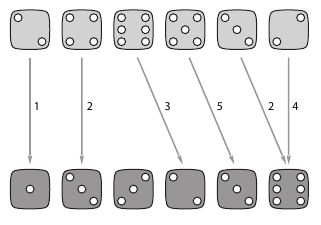
\includegraphics[scale=1]{pics/kubiki}
\label{pic:kubiki}
\caption{Две линии из шести игральных кубиков, с соответственными частичными суммами.}
\end{figure}

По построению, $\alpha_m-\beta_{m'}\ge 0$;
заметим, что эта разница не превышает $n-1$ 
(если $\alpha_m-\beta_{m'}\ge n$, то индекс $m'$ не максимален).
Если какая-то из разниц $\alpha_m-\beta_{m'}$ равна $0$, то задача решена --- в этом случае, взяв $j=s=1$, $k=m$ и $t=m'$, получим два начальных сегмента с одинаковыми суммами.
Если же ни одна из разниц $\alpha_m-\beta_{m'}$ не равна $0$, то все $n$ разниц 
$\alpha_m-\beta_{m'}$ лежат в множестве $\{1,\dots,n-1\}$ и, значит, две из них равны.
Предположим, что это $\alpha_p-\beta_{p'}$ и $\alpha_q-\beta_{q'}$.
Но тогда 
\[\sum_{i=p+1}^qa_i=\sum_{i=p'+1}^{q'}b_i.\]
--- снова победа.

Ну ведь очень хитр\'{о}?

На рисунке есть только одна пара совпадающих разностей (обе равны 2), а именно $p=2$, $q=5$, $p'=2$ и $q'=6$;
вот соответственные подстроки с равными суммами:
\[a_3+a_4+a_5=6+5+3=3+2+3+6=b_3+b_4+b_5+b_6.\]

\begin{addedbytheeditors}
У этой идеи есть и другие применения; иногда неожиданные как например следующий результат \cite{petrunin}:
\textit{Пусть $\tilde M\to M$ есть $n$-листное локально-изометрическое накрытие компактного риманова многообразия $M$.
Тогда $\mathrm{diam}\, \tilde M\le n\cdot \mathrm{diam}\, M$}, где $\mathrm{diam}\, M$ обозначает диаметр $M$ то есть максимальное расстояние между парой точек в $M$.
\end{addedbytheeditors}
